\documentclass{nslsii}
\usepackage{graphicx}

\usepackage{hyperref}

\title{\LaTeX{}  for NSLS II Technical Notes}
\author{D. Hidas}
\date{\today}
\notenumber{1234}

\begin{document}

\maketitle

\begin{abstract}
This is an example of how get and to use the nslsii \LaTeX{} class to produce an NSLS II Technical Note.
\end{abstract}



\section{Availability}
You can clone the repository \href{https://github.com/dhidas}{https://github.com/dhidas}:
\begin{verbatim}
> git clone https://github.com/dhidas/asd.git
\end{verbatim}

\section{Usage}
Edit Template.tex, nslsii.cls, and Makefile as you see fit.  Typically to compile the example one only needs to:
\begin{verbatim}
> make
\end{verbatim}
which will generate Template.pdf


\section{Contribute}
Please contribute improvements to the repository for everyone to enjoy.


\section{Figures}
It is nice to throw in a figure such as figure~\ref{fig:example} and some math
$$
\vec E(\vec r, \omega) = \frac{ie\omega}{4 \pi c \epsilon_0} \int_{-\infty}^{+\infty} \frac{\vec \beta - \hat n (1 + \frac{i c}{ \omega D})}{D} e^{i \omega ( \tau + \frac{D}{c} )} d\tau
$$

\begin{figure}
\centering
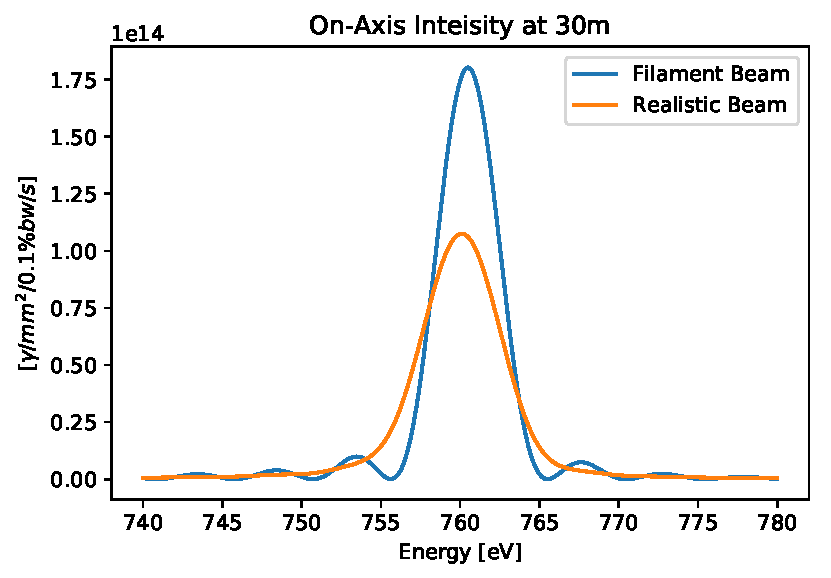
\includegraphics[width=0.5\columnwidth]{img/spectra}
\caption{Example figure caption goes here.  This plot was created with matplotlib~\cite{bib:matplotlib}}.
\label{fig:example}
\end{figure}


\section*{Acknowledgement}
Thanks mostly to internet search engines and previous \LaTeX{} survivors.





\begin{thebibliography}{00}

\bibitem{bib:matplotlib}
J.~D.~Hunter, “Matplotlib: A 2D graphics environment,”
in Computing In Science and Engineering vol 9 n 3, 2007


\end{thebibliography}

\end{document}
